在本次课程项目的实践过程中,发现了许多想象中没有出现的问题,并且通过搜索了很多资料,找到了许多方法压缩代码,节省时间,压缩内存空间。例如:

\subsection{编程技巧}

\subsubsection{宏定义与头文件规范}

定义时,我总希望能够使得main.cpp显得不那么冗杂,所以希望开启新的config.h来搜集一切宏定义和全局变量。

搜索资料后发现,头文件通常用于声明变量,而不是定义变量。对于全局变量,应该在头文件中使用extern关键字来声明,然后在一个源文件中实际定义。
并且注释部分的信息(如创建者信息和联系方式)最好放在实现文件(.cpp)中,而不是头文件中。

\subsubsection{宏定义与构造函数接口的冲突}

在使用MQUnifiedsensor.h库时,public接口如下所示:

\texttt{MQUnifiedsensor(String Placa = "Arduino", float Voltage\_Resolution =  5, int ADC\_Bit\_Resolution = 10, int pin = 1, String type = "CUSTOM MQ");}

我在configuration.h中使用\texttt{\#define Voltage\_Resolution 3.3},出现以下报错:

\begin{lstlisting} 
    : note: in expansion of macro 'Voltage_Resolution'
     MQUnifiedsensor(String Placa = "Arduino", float Voltage_Resolution =  5, int ADC_Bit_Resolution = 10, int pin = 1, String type = "CUSTOM MQ");
\end{lstlisting}

报错原因:宏定义是字符替换,这里编译时会变成 "3.3 = 5",故导致编译错误。

\subsubsection{使用"F"宏处理字符串}

F()宏:当使用F()宏时,字符串常量会存储在Flash存储器中,而不是默认的SRAM中。这意味着可以减少动态内存的使用,提高程序的运行效率。
如果不使用F()宏,所有字符串常量(例如"Humidity: ")都会存储在SRAM中。对于内存较少的设备(如Arduino Uno)来说,这会迅速消耗有限的SRAM,导致“内存不足”错误。

参考资料:\href{https://blog.csdn.net/fang\_chuan/article/details/80029546}{\underline{https://blog.csdn.net/fang\_chuan/article/details/80029546}}

使用正则表达式将println\textbackslash("([\textasciicircum"]*)"\textbackslash)替换为println(F("\$1"))即可。

\subsubsection{PlatformIO Libraries 处理方案}

在Arduino IDE上编辑时,库是容易导入的,但对于大文件和项目组织的管理,Arduino IDE的表现令人不满。
于是我选择转向了VSCode + Platform 开发,但Clion中许多VSCode没有的功能更加吸引我,所以转向了Jetbrains家族。

但是初次接触时,我被其复杂性所惊讶,在互联网上搜索相关的导入库的教程也是少之又少,迫不得已到StackOverflow上搜索,并将部分优秀结果自我吸收后作了整理写入了个人的bilibili专栏。

阅读链接:\href{https://www.bilibili.com/read/cv37521671}{\underline{www.bilibili.com/read/cv37521671}}

\subsubsection{ESP32 崩溃后使用 Backtrace 追踪错误代码}

在上传后,有时会出现如下的报错:

\begin{figure} [H]
    \centering
    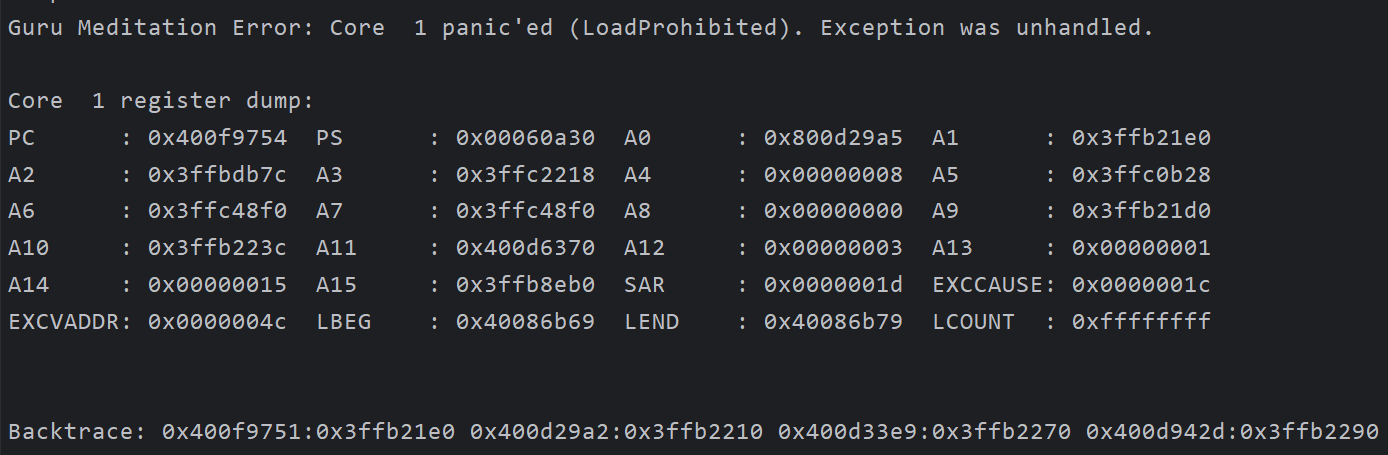
\includegraphics[width=0.5\textwidth]{img/ESP32Error.png}
    \caption{ESP32 崩溃}
    \label{fig:ESP32_crash}
\end{figure}

通过查找资料,可以使用ESP32自带的工具:xtensa-esp32s3-elf-gcc来追溯源代码

命令如下:
\begin{lstlisting}
PS C:\Users\26421\AppData\Local\Arduino15\packages\esp32\tools\xtensa-esp32s3-elf-gcc\esp-2021r2-patch5-8.4.0\bin> .\xtensa-esp32s3-elf-addr2line -pfiaC -e C:\Users\26421\Desktop\Maker\Slave\.pio\build\upesy_wroom\firmware.elf 0x400d29a2:0x3ffb2210 0x400d33e9:0x3ffb2270 0x400d942d:0x3ffb2290
\end{lstlisting}

其中,-e参数指定了elf文件路径,0x400d29a2:0x3ffb2210 0x400d33e9:0x3ffb2270 0x400d942d:0x3ffb2290分别是三个崩溃点的地址。
效果如下所示:

\begin{figure} [H]
    \centering
    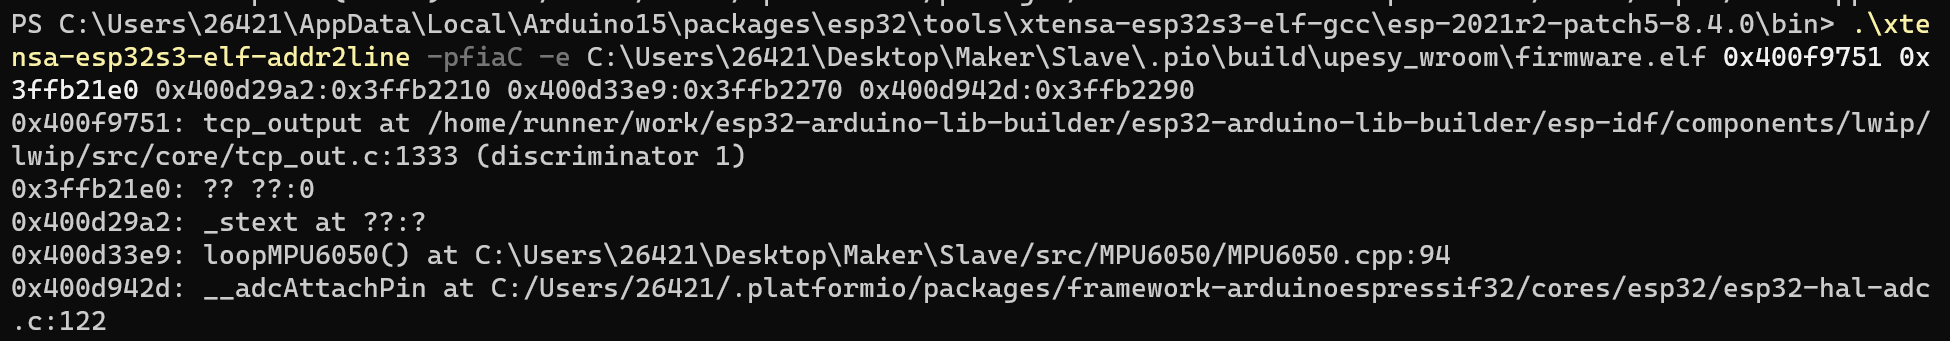
\includegraphics[width=0.7\textwidth]{img/ESP32Backtrace.png}
    \caption{ESP32 Backtrace 追踪错误代码}
    \label{fig:ESP32_backtrace}
\end{figure}


\subsection{个人体验}

本项目乃是我大一一整年做过体量最大、投入最多的项目,很感谢创客实践让我从对嵌入式一窍不通到变得感兴趣。
几乎一切都是从零开始,觉得最有挑战性的部分是涉及到舵机、机械结构的运动学解算,这一部分是需要和外校的同学交流后才知道的。
最觉得有收获的部分是,一点一点地实现语音输入和语音识别、到最后TTS模块的成功运用。

那么,有了语音识别之后,可以再做一些什么呢?不如加一些传感器读取一下个人身体上、房间内、城市里的各种参数吧!
语音识别和输出,显然可以让生活更智能,在项目的构建过程中,也越来越体会到框架的美感。
还有将函数重写时,变得简约易读的程序员之美,在完成一切工作后都体现得淋漓尽致!

为了做一个更漂亮的排版,我去学习了LateX,为了更好的编程和组织文件,我去学习了PlatformIO,最后为了尝试更多东西,跨入了SolidWorks的门槛。
在学习的过程中也接触了很多新概念和新玩法,例如卡尔曼滤波、sha256算法,API的鉴权处理,甚至到ws协议和wss协议的区别。

由于本人在家中尝试搭建家中的路由器组网,所以对网络的了解也更深了一层,能够很快切入ESP32的$AC+AP$模式,甚至有了用ESP32构建Mesh网络的想法。

当然,由于很多部分是第一次探索,搜索了很多资料,也不缺少对各种大模型的使用,但在使用大模型的同时,我将大模型部署到了本地,也许这本身更让人愉悦。
为什么要去实现本来看起来很困难的事情,因为山就在那里。

\subsection{未来设想}

CSI(Channel State Information)用于描述无线通信中的信道特性,可以反映出无线信号在传播过程中受到的多径、衰减、干扰等影响。CSI 在 Wi-Fi 系统中广泛应用,尤其是基于 OFDM(正交频分复用)技术的 Wi-Fi 标准,如 802.11n/ac/ax。
在这些标准中,CSI 可以用于优化传输性能、定位和环境感知等应用。

南京大学无线感知前沿技术论坛在8月1日分享了CSI的前沿研究成果,有望实现毫米级的动态感应。
参考链接:\href{https://www.bilibili.com/video/BV1Cv411q7Cz}{\underline{https://www.bilibili.com/video/BV1Cv411q7Cz}}
,这一部分已有人通过算法实现,原理如同切割磁感线一般,可以通过Wifi强度在人为动作后感应信道的变化,从而读取人类活动,应用前景广泛,将来我很可能从事这方面的研究。

参考链接:\href{https://www.bilibili.com/video/BV1cGHreYEzB}{\underline{用 ESP32-S3 和 CSI 技术打造人体感知风扇}}

\begin{figure} [H]
    \centering
    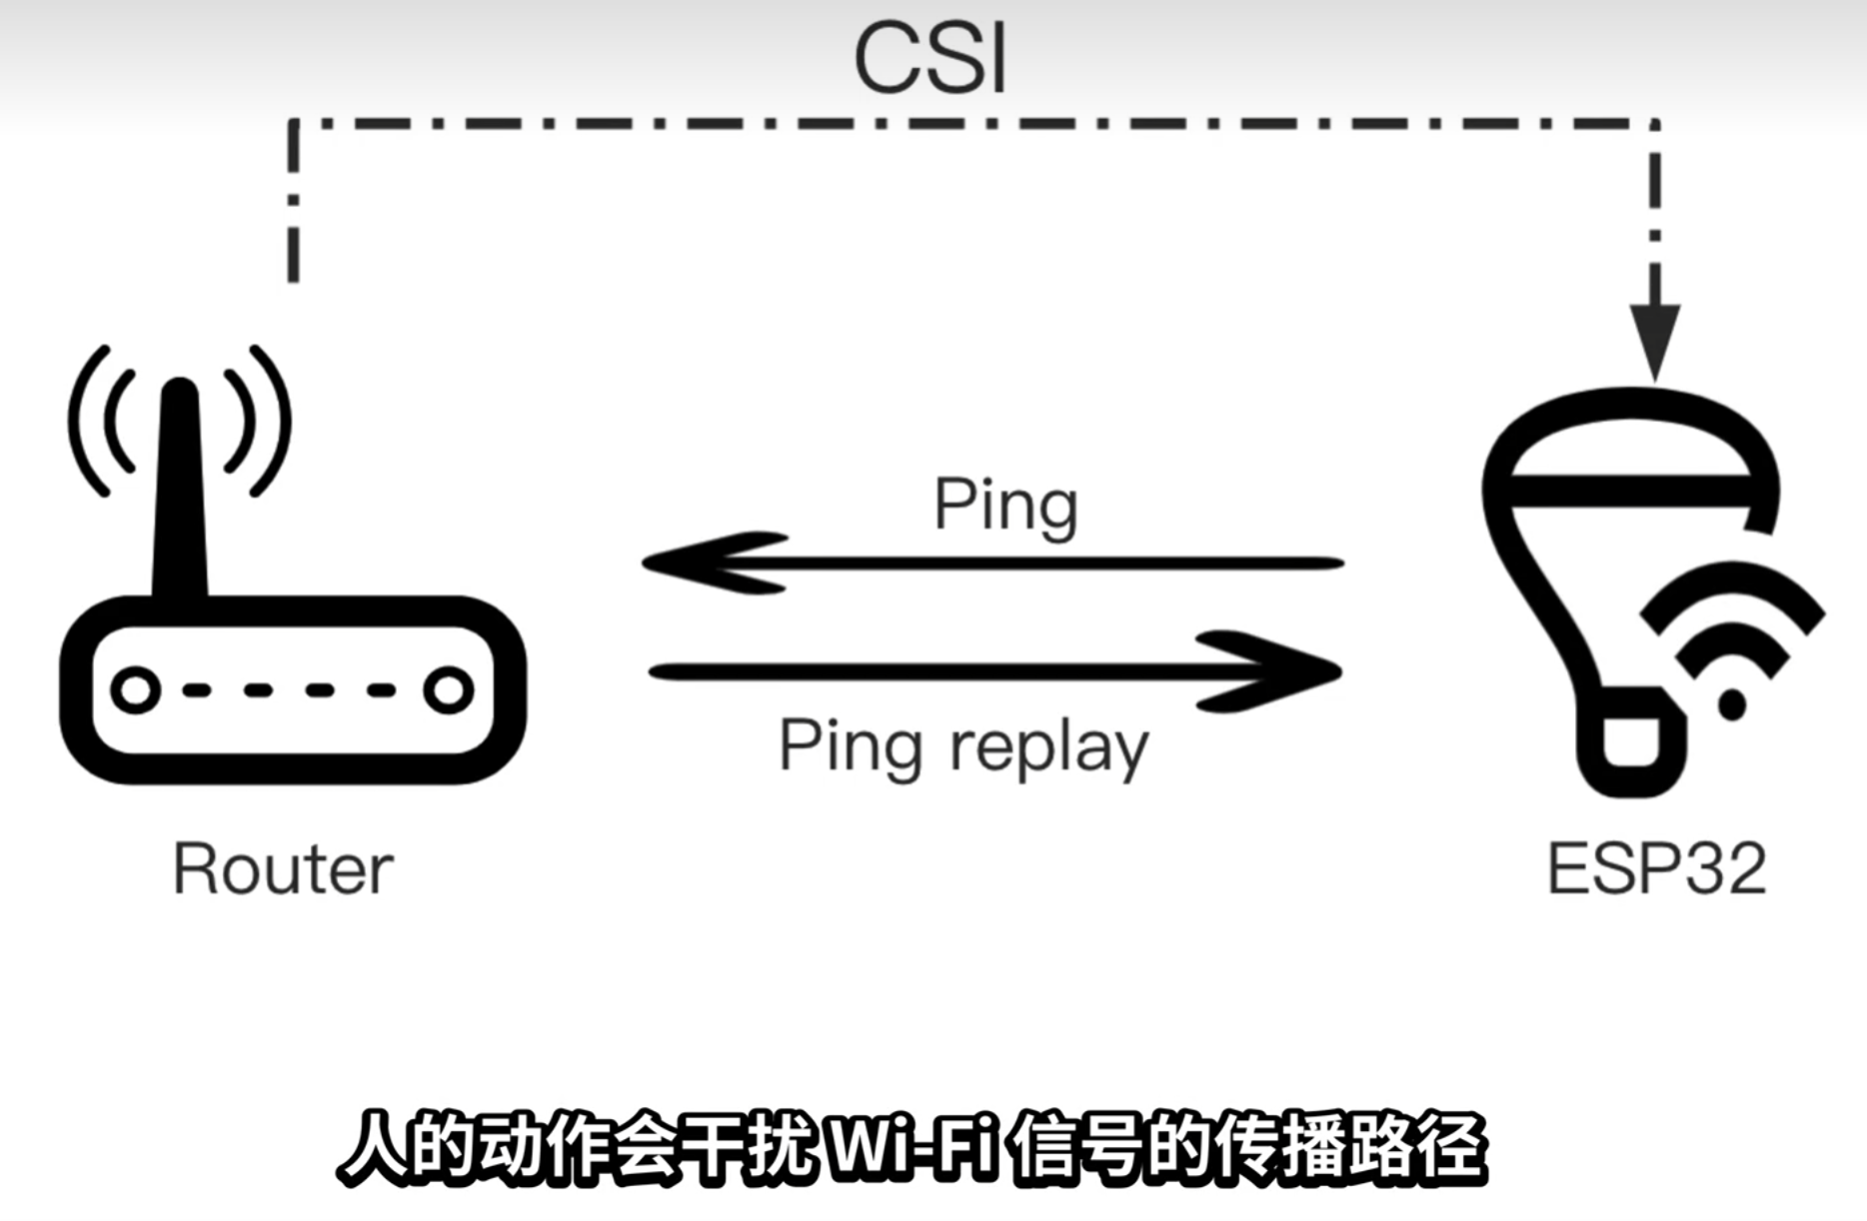
\includegraphics[width=0.4\textwidth]{img/CSI.png}
    \caption{CSI与ESP32-S3结合示意图}
    \label{fig:CSI}
\end{figure}